\section{Dataset and Reservoir Description}
The underground hydrogen storage (UHS) surrogate models are developed and validated using a dataset comprising five independent reservoir simulation cases, each representing a two-year cyclic storage operation. The reservoir geometry is discretized on a two-dimensional, irregular Perpendicular Bisection (PEBI) / Voronoi grid containing 10,116 active control cells. Cell centroid coordinates span $X_i \in [12.5,\, 4987.5]$~m laterally and $Z_i \in [0.25,\, 99.75]$~m in depth. Each simulation run yields 146 dynamic state snapshots recorded at a uniform reporting interval of five days, representing 730 days of cumulative operating time. Across the five cases, the absolute permeability field realizations and well schedules are systematically varied; details of the geostatistical parameters and schedule ranges are maintained in the project data specifications.

A spatial-temporal overview of the cyclic well operating schedules and the resulting average reservoir pressure is shown in Fig.~\ref{fig:dataset_overview}, while the centroid layout of the native irregular mesh and well positions is illustrated in Fig.~\ref{fig:mesh_topology}. The spatial-temporal pressure field snapshots across representative operating phases (injection, shut-in, and production) are visualized in Fig.~\ref{fig:pressure_evolution}.

\begin{figure*}[t]
    \centering
    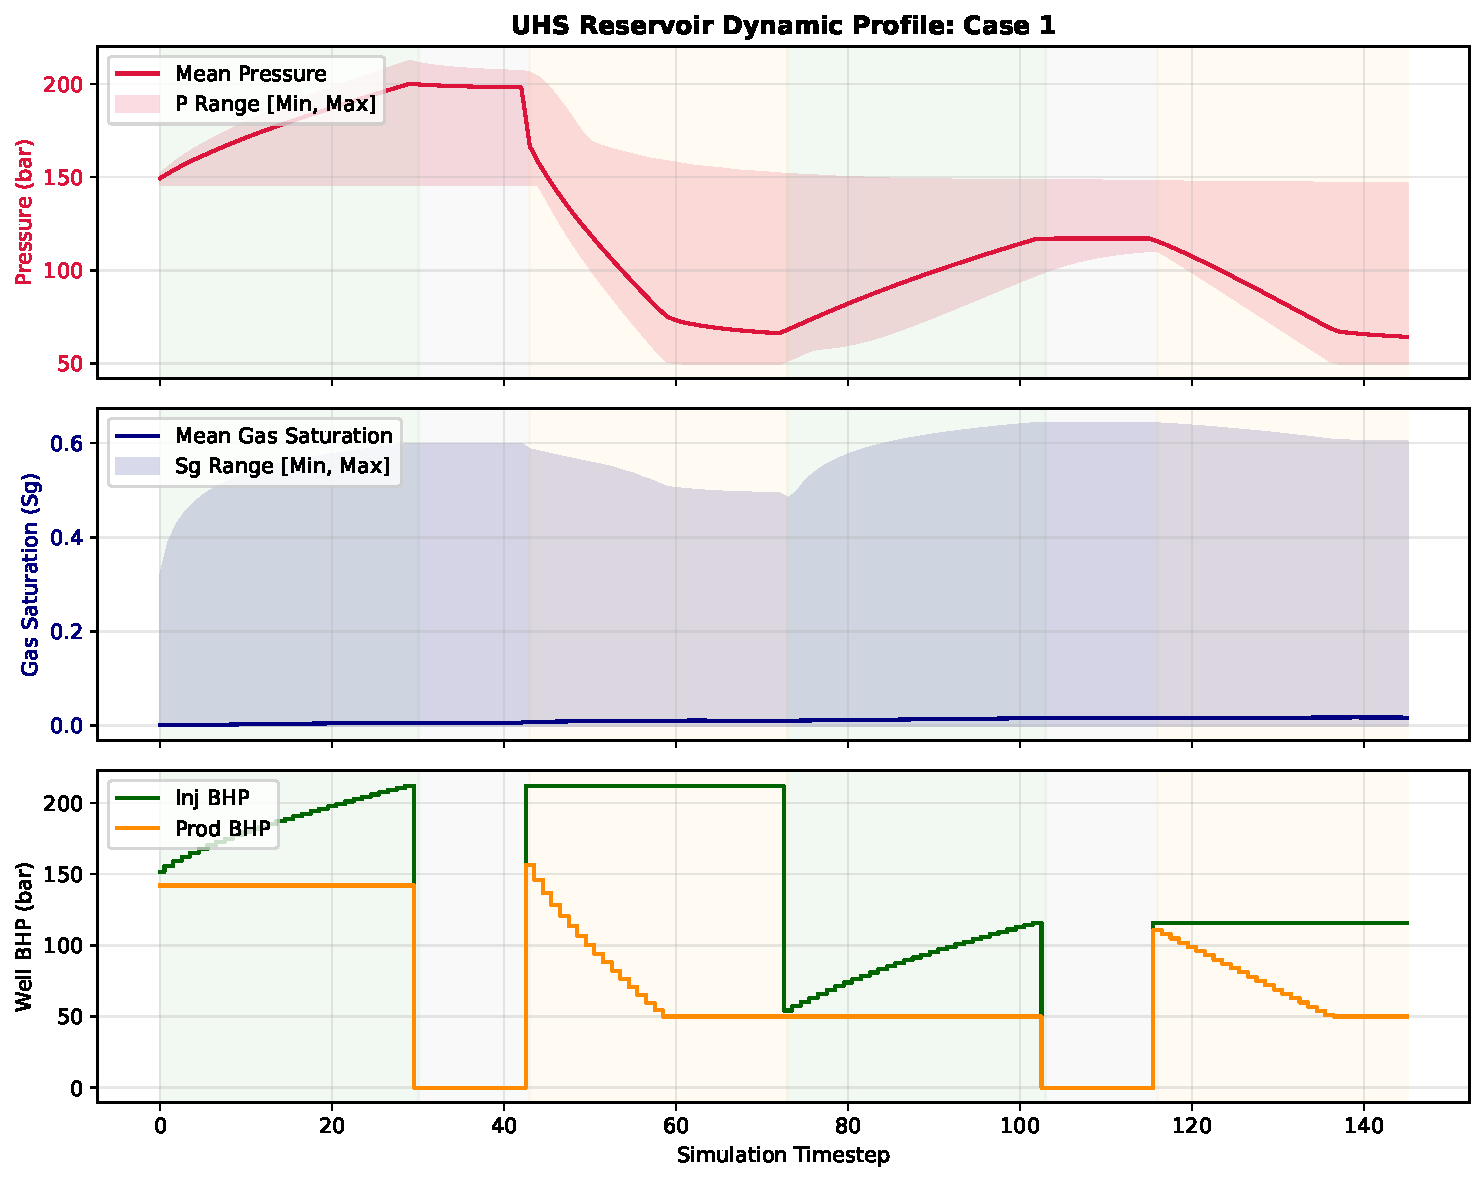
\includegraphics[width=\textwidth]{figures/fig1_dataset_overview}
    \caption{Overview of the Underground Hydrogen Storage (UHS) dataset, showing typical cyclic well operating schedules (injection/production BHP and flow rates) and the resulting average reservoir pressure over a 730-day (2-year) timeline.}
    \label{fig:dataset_overview}
\end{figure*}

\begin{figure}[htbp]
    \centering
    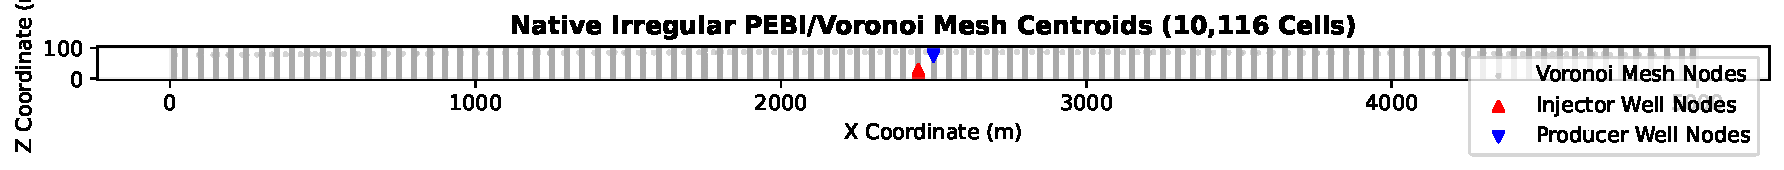
\includegraphics[width=0.95\columnwidth]{figures/fig2_mesh_topology}
    \caption{Centroid coordinate distribution of the native 10,116-cell irregular PEBI/Voronoi mesh, highlighting the locations of the injector (red triangles) and producer (blue triangles) well centroids.}
    \label{fig:mesh_topology}
\end{figure}

\begin{figure*}[t]
    \centering
    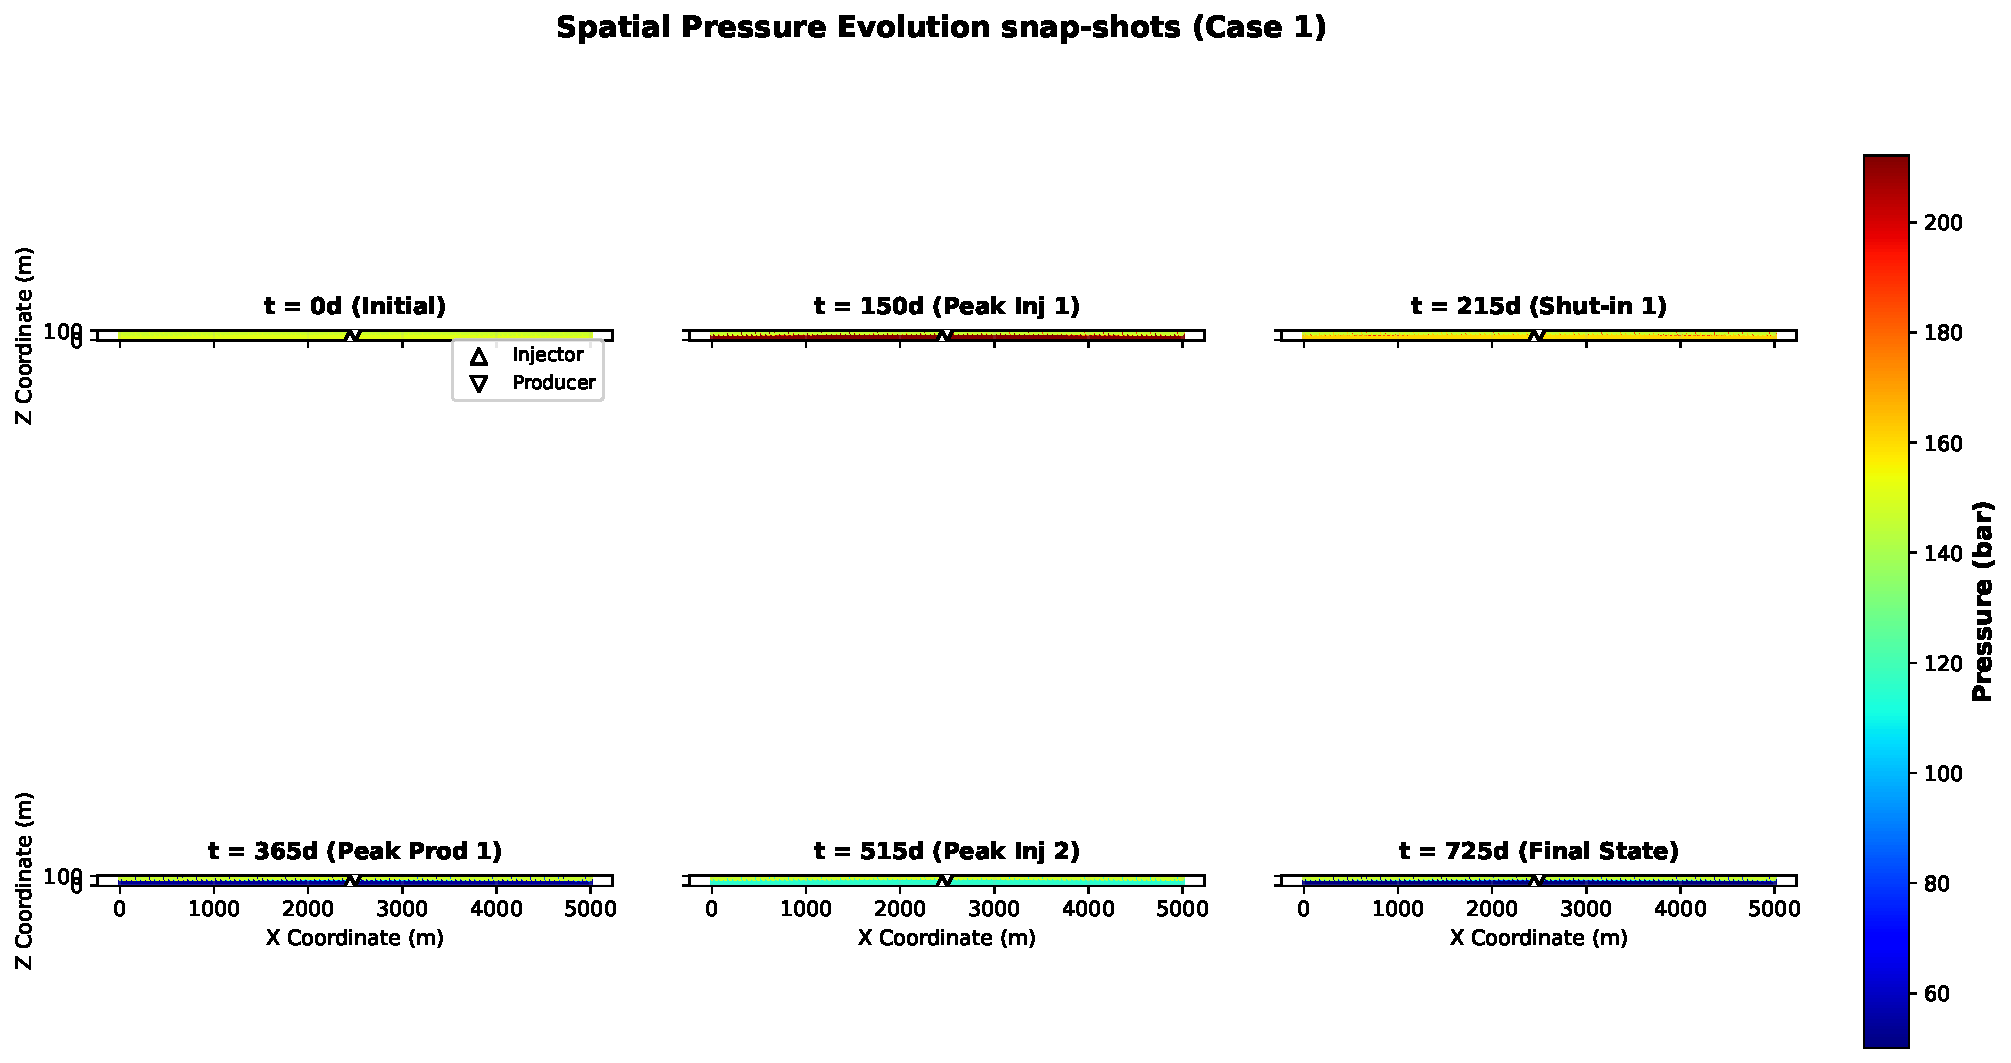
\includegraphics[width=\textwidth]{figures/fig3_pressure_evolution}
    \caption{Dynamic spatial pressure snapshots (bar) at representative timesteps during injection, shut-in, and production phases of Case 1, highlighting localized transient pressure gradients near the wellbores.}
    \label{fig:pressure_evolution}
\end{figure*}

\subsection{Variables and Operational Cycles}
Each simulation case tracks 46 physical and biological quantities, of which the following subset is utilized for surrogate modeling:
\begin{itemize}
    \item \textbf{Spatio-Temporal State Matrices} ($10,116 \times 146$): Cell-wise pressures $P_i(t)$, gas phase saturations $S_{g,i}(t)$, water phase saturations $S_{w,i}(t)$, and hydrogen mole fractions in the vapor ($y_{\text{H}_2, i}(t)$) and liquid ($x_{\text{H}_2, i}(t)$) phases.
    \item \textbf{Dynamic Well Controls} ($1 \times 146$ per well): Bottomhole pressure (BHP) targets and volumetric injection/production rates for both the injector and producer wells.
    \item \textbf{Static Rock Properties} ($10,116 \times 1$): Initial porosity $\phi_i$, absolute permeability $k_i$, and centroid coordinates $(X_i, Z_i)$.
\end{itemize}

The operational schedule in each simulation consists of a cyclic injection-withdrawal protocol: active H$_2$ injection occurs during steps 1--60, followed by a shut-in period during steps 61--86, and active gas production during steps 87--146. Operating well control transitions occur at step indices 30, 73, and 103 for the injector well, and at indices 43, 73, and 116 for the producer well. These transition steps induce highly transient pressure transients that challenge data-driven emulators.

\subsection{Train/Test Split and Standardization}
To evaluate model performance, Cases 1--4 (comprising 584 timesteps and 10,116 cells) are designated as the training set, while Case 5 is held out as an independent test set. This temporal split assesses whether the model can emulate a complete, unseen cyclic storage trajectory under a novel geostatistical permeability realization. It is important to note that this evaluation represents interpolation within a controlled geostatistical parameter space rather than extrapolation to unseen geological topologies.

To prevent data leakage, Z-score standardization parameters ($\mu_{\text{train}}, \sigma_{\text{train}}$) are computed exclusively from Cases 1--4 and applied to the test set. Because the timestep size ($\Delta t = 5$~days) remains constant, it contains zero variance and is excluded from feature scaling. The normalization statistics for the raw input features are summarized in Table~\ref{tab:dataset_stats}.

\begin{table*}[t]
\centering
\caption{Dataset Variable Normalization Parameters (Cases 1--4)}
\label{tab:dataset_stats}
\begin{tabularx}{\linewidth}{lXcc}
\toprule
\textbf{Feature Name} & \textbf{Physical Meaning} & \textbf{Mean ($\mu_{\text{train}}$)} & \textbf{Std Dev ($\sigma_{\text{train}}$)} \\
\midrule
`Perm` & Absolute Permeability (mD) & 203.3158 & 209.8465 \\
`Poro` & Rock Porosity (fraction) & 0.1076 & 0.0249 \\
`P(t)` & Pressure at step $t$ (bar) & 120.7029 & 50.7625 \\
`inj\_BHP` & Injection Well BHP (bar) & 122.6423 & 74.1365 \\
`prod\_BHP` & Production Well BHP (bar) & 69.9383 & 49.0101 \\
`inj\_H2` & Injection H$_2$ Rate (daily rate units) & 3.5269 & 4.1979 \\
`prod\_H2` & Production H$_2$ Rate (daily rate units) & 2.2432 & 3.5813 \\
`dt\_days` & Time step size (days) & 5.0000 & 0.0000 \\
`t\_index` & Time step index (dimensionless) & 72.0000 & 41.8569 \\
\bottomrule
\end{tabularx}
\end{table*}

